\documentclass[12pt]{article}

% Language setting
\usepackage[utf8]{inputenc}
\usepackage[bulgarian]{babel}

% --------------------- Packages  --------------------
% Use biblatex
\usepackage{biblatex}
\addbibresource{bibliography.bib}
% Table thickness
\usepackage{ctable}
% Equations: SI units
\usepackage{siunitx}
% Approximately equal
\usepackage{amssymb}
% degrees symbol
\usepackage{gensymb}
% warning box
\usepackage{pifont,mdframed}
% Multiline math
\usepackage{amsmath}

\newenvironment{warning}
  {\par\begin{mdframed}[linewidth=2pt, linecolor=white]%
    \begin{list}{}{\leftmargin=1cm
                   \labelwidth=\leftmargin}\item[\Large\ding{43}]}
  {\end{list}\end{mdframed}\par}

% --------------------- Title  --------------------
\addbibresource{bibliography.bib}

\begin{document}

% Anfang der Titelseite________________________________________________________________________________
\begin{titlepage}
	\flushleft
	{\scshape\Large Протокол I \hspace{2cm} Молекулна физика\par}
	\vspace{4cm}
	{\huge\bfseries Коефициент на повърхностно напрежение\par}
	\vspace{1cm}
	{\LARGE\bfseries Лабораторно упражнение №3.6\par}
	\vspace{5cm}
    {\LARGE\bfseries Виолета Кабаджова, \par}
    {\large\bfseries ККТФ, фак. номер: 3PH0600026\par}
	\vspace{1cm}
	
	{\large Физически Факултет, 
	
	Софийски Университет "Св. Климент Охридски"
	
	02 юни 2023 г.\par}
	
\end{titlepage}

\section{Теоритична част}\label{sec:theoretical-part}
Всяка молекула взаимодействша само с тези, намиращи се в нейния т.нар. радиус на междумолекулно взаимодействие, равняващ се на най-много няколко ефективни диаметъра на молекулата.

Нека изследваме молекули на течност в равновесно състояние, разположени както е показано на фиг. \ref{fig:cohesion-forces}. Около изследваниете молекули са начертани радиусите на междумолекулно взаимодействие, заедно с молекулите, с които изследваната влиза в контакт. Поради еднаквата плътност на течността във всички посоки и немалкият брой взаимодействащи молекули в околността на молекулите, разположени във вътрешността на течността, им действат сили равномерно във всички посоки и равнодействащата на тези сили е нула. На молекулите, разположени на повърхността на течността обаче, им действат много повече сили на привличане навътре към течността отколкото силите на привличане извън нея, поради много по-ниската плътност на въздуха спрямо тази на течността. Резултатната на тези сили наричаме кохезионна сила и тя е перпендикулярна на повърхността на течността и насочена към вътрешността ѝ. Големината ѝ е по-голяма за молекулите, намиращи се точно на граничния слой на течността, спрямо тези, намиращи се по-навътре в течността.

\begin{figure}
    \centering
    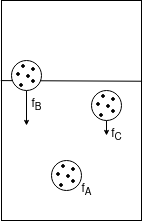
\includegraphics[width=0.2\textwidth]{images/cohesion-forces.png}
    \caption{\label{fig:cohesion-forces} Към извод за кохезионни сили}
\end{figure}

В повърхностния слой се установява състояние на динамично равновесие, което означава, че във всеки момент молекулите преминаващи от повърхностния слой към обема на течността е равен на молекулите, движещи се в обратна посока. Поради кохезионните сили първия начин е много по-лесен, което води до това, че, за да може системата да влезе в състояние на динамично равновесие, е необходимо броят на молекулите в повърхностния слой да е много по-малък. Поради това той се явява като "разтегнат" слой на течността и се появяват сили, противопоставящи се на тази деформация, наречени сили на повърхностно напрежение. Големината на тази сила, отнесена към единица дължина от контура наричаме коефициент на повърхностно напрежение $\sigma$, [$\sigma$] = $N/m$ (ур. \ref{eq:sigma-1}). 

\begin{equation}\label{eq:sigma-1}
    \sigma = \frac{f_\sigma}{l}
\end{equation}

Поради факта, че, за да се придвижи една молкула от граничния слой към обема на течността, е необходимо да се извърши работа, то в повърхностния слой възниква потенциална енергия $U_{s}$ (от $U_{surface}$), пропорционална на повърхността $S$ на течността, откъдето може да се даде и нова дефиниция за $\sigma$ - ур. \ref{eq:sigma-2}, [$\sigma$] = $J/m^2$.

\begin{equation}\label{eq:sigma-2}
    \sigma = \frac{U_s}{S}
\end{equation}

Трета дефиниция, която може да се даде на $sigma$ включва работата $\delta A$, която трябва да се извърши при $T=$const, за да се измени свободната повърхност с $dS$:

\begin{equation}
    \delta A = -dU_s = -\sigma dS,
    \sigma = -\frac{\delta A}{dS}
\end{equation}

\section{Експериментална част}

\subsection{Експериментална установка}
\begin{figure}
    \centering
    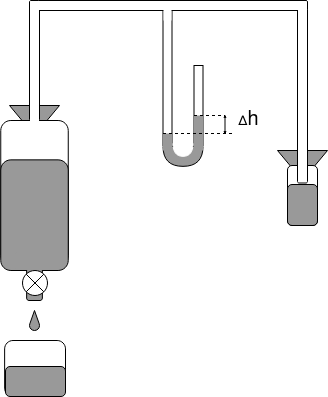
\includegraphics[width=0.5\textwidth]{images/surface-tension-setup.png}
    \caption{\label{fig:setup}Схема на опитна постановка}
    \label{fig:setup}
\end{figure}

На фиг. \ref{fig:setup} в бурканчето, разположено вдясно, се поставя последователно спирт 10\%, 20\%, 30\%, 40\%, 50\%, течност с неизвестно съдържание на спирт X\% и дестилирана вода, които изследваме едно след друго. Капилярката е така поставена, че едва да докосва повърхността на изследваната течност. Когато крана на аспиратора (най-вляво на фигурата) се отвори леко, поставената в него вода, започва да тече под формата на капчици. Това предизвиква разлика в налягането, което води до оформяне на капчица в излседваната течност. Отчита се максималната стойност на $\Delta h$ в диференциалния манометър при постоянно отделяне на мехурчета в течността. 

Поради капилярните свойства, течността в капилярката се изкриявава (вдлъбната или изпъкнала). Промяната на налягането под изкривената сферична повърхност се дава от формулата на Лаплас - ур. \ref{eq:laplace-formula}, където $R$ - радиуса на повърхността. Стойността е положителна, когато повърхността е изпъкнала, и отрицателна в обратния случай.

\begin{equation}\label{eq:laplace-formula}
    \Delta p = \pm \frac{2\sigma}{R}
\end{equation}

Когато течността мокри капилярката, повърхността ѝ е вдлъбната ($\Delta p$ < 0). Тогава налягането под повърхността на течността в капилярката намалява (ур. \ref{eq:p-1}) - $p_{atm}$ - атмосферно налягане, $R$ - радиус на капилярката. За да се компенсира разликата в налягането, течността в капилярката се издига на височина $h$ и създава допълнително хидростатично налягане $\rho_Tgh$, където $\rho_T$ е плътността на изследваната течност (ур. \ref{p-2}), откъдето следва уравнение \ref{eq:p-3}. 

\begin{equation}\label{eq:p-1}
    p = p_{atm} - \frac{2\sigma}{R}
\end{equation}

\begin{equation}\label{eq:p-2}
    p_{atm} = p + \rho_Tgh
\end{equation}

\begin{equation}\label{eq:p-3}
    \frac{2\sigma}{R} = \rho_Tgh
\end{equation}

Формула \ref{eq:laplace-formula} ни дава точната граница на налягане, диференциално малко след която се откъсва мехурче от капилярката, следователно \ref{eq:p_min}. Диференциалният манометър измерва $p_{atm} - p_{min} = \rho g \Delta h$, където $\rho$ е плътността на течността в манометъра, а $\Delta h$ - разликата във височините на двете колена на манометъра. Тогава за коефициента на вътрешно напрежение се получава формула \ref{eq:result}.

\begin{equation}\label{eq:p-min}
    p_{min} = p_{atm} - \frac{2\sigma}{R}
\end{equation}

\begin{equation}\label{eq:result}
    \sigma = R\frac{\rho g \Delta h}{2}
\end{equation}

\subsection{Задача: Измерване на коефициента на повърхностно напрежение на разствор на спирт и вода с различни концентрации по абсолютния метод}

Използваме формула \ref{eq:result}, за да открием $\sigma$, като грешката оценяваме отгоре чрез формула \ref{eq:abs-err}. Резултатите записваме в таблици \ref{tbl:results-10} до \ref{tbl:constants} включително.

\begin{equation}\label{eq:abs-err}
    \Delta \sigma = \sigma\left[\frac{\Delta R}{R} + \frac{\Delta \rho}{\rho} + \frac{\Delta g}{g} + \frac{\Delta (\Delta \bar{h})}{\Delta \bar{h}}\right]
\end{equation}


\begin{table}[h]
\begin{center}
\begin{tabular}{|l|l|l|}
\specialrule{.1em}{0em}{0em}
N & $\Delta h$, [cm] & $(h_i - \bar{h})^2$ \\ \hline
\specialrule{.1em}{0em}{0em}
1 &3.5 &0.0196 \\ \hline
2 &3.8 &0.0256 \\ \hline
3 &3.5 &0.0196 \\ \hline
4 &3.5 &0.0196 \\ \hline
5 &3.9 &0.0676 \\ \hline
\specialrule{.1em}{0em}{0em}
$\Delta \bar{h}$ & (3.64 $\pm$ 0.35) \cdot 10$^{-2}$ m & $\Delta \Delta h/\Delta h = 0.10$\\ \hline
$\sigma$ & 0.501 $\pm$ 0.049 N/m & $\Delta \sigma/\sigma = 0.10$  \\ 
\specialrule{.1em}{0em}{0em}
\end{tabular}
\caption{\label{tbl:results-10}Измервания и резултати - разтвор 10\%}
\end{center}
\end{table}

\begin{table}[h]
\begin{center}
\begin{tabular}{|l|l|l|}
\specialrule{.1em}{0em}{0em}
N & $\Delta h$, [cm] & $(h_i - \bar{h})^2$ \\ \hline
\specialrule{.1em}{0em}{0em}
1 & 3.5 & 0.0676 \\ \hline
2 & 3.1 & 0.0196 \\ \hline
3 & 3.3 & 0.0036 \\ \hline
4 & 3.3 & 0.0036 \\ \hline
5 & 3.0 & 0.0576 \\ \hline
\specialrule{.1em}{0em}{0em}
$\Delta \bar{h}$ & (3.24 $\pm$ 0.35) \cdot 10$^{-2}$ m & $\Delta \Delta h/\Delta h = 0.10$\\ \hline
$\sigma$ & 0446 $\pm$ 0.049 N/m & $\Delta \sigma/\sigma = 0.11$  \\ 
\specialrule{.1em}{0em}{0em}
\end{tabular}
\caption{\label{tbl:results-20}Измервания и резултати - разтвор 20\%}
\end{center}
\end{table}

\begin{table}[h]
\begin{center}
\begin{tabular}{|l|l|l|}
\specialrule{.1em}{0em}{0em}
N & $\Delta h$, [cm] & $(h_i - \bar{h})^2$ \\ \hline
\specialrule{.1em}{0em}{0em}
1 & 2.6 & 0.0036 \\ \hline
2 & 2.7 & 0.0256 \\ \hline
3 & 2.5 & 0.0016 \\ \hline
4 & 2.5 & 0.0016 \\ \hline
5 & 2.4 & 0.0196 \\ \hline
\specialrule{.1em}{0em}{0em}
$\Delta \bar{h}$ & (2.54 $\pm$ 0.20) \cdot 10$^{-2}$ m  & $\Delta \Delta h/\Delta h = 0.08$ \\ \hline
$\sigma$ & 0.400 $\pm$ 0.029 N/m & $\Delta \sigma/\sigma = 0.08$  \\ 
\specialrule{.1em}{0em}{0em}
\end{tabular}
\caption{\label{tbl:results-30}Измервания и резултати - разтвор 30\%}
\end{center}
\end{table}

\begin{table}[h]
\begin{center}
\begin{tabular}{|l|l|l|}
\specialrule{.1em}{0em}{0em}
N & $\Delta h$, [cm] & $(h_i - \bar{h})^2$ \\ \hline
\specialrule{.1em}{0em}{0em}
1 & 2.1 & 0.0784 \\ \hline
2 & 2.4 & 0.0004 \\ \hline
3 & 2.6 & 0.0484 \\ \hline
4 & 2.4 & 0.0004 \\ \hline
5 & 2.4 & 0.0004 \\ \hline
\specialrule{.1em}{0em}{0em}
$\Delta \bar{h}$ & (2.38 $\pm$ 0.32) \cdot 10$^{-2}$ m & $\Delta \Delta h/\Delta h = 0.14$ \\ \hline
$\sigma$ & 0.328 $\pm$ 0.045 N/m & $\Delta \sigma/\sigma = 0.14$  \\ 
\specialrule{.1em}{0em}{0em}
\end{tabular}
\caption{\label{tbl:results-40}Измервания и резултати - разтвор 40\%}
\end{center}
\end{table}

\begin{table}[h]
\begin{center}
\begin{tabular}{|l|l|l|}
\specialrule{.1em}{0em}{0em}
N & $\Delta h$, [cm] & $(h_i - \bar{h})^2$ \\ \hline
\specialrule{.1em}{0em}{0em}
1 & 2.1 & 0.0144 \\ \hline
2 & 2.3 & 0.0064 \\ \hline
3 & 2.1 & 0.0144 \\ \hline
4 & 2.3 & 0.0064 \\ \hline
5 & 2.3 & 0.0064 \\ \hline
\specialrule{.1em}{0em}{0em}
$\Delta \bar{h}$ & (2.22 $\pm$ 0.20) \cdot 10$^{-2}$ m & $\Delta \Delta h/\Delta h = 0.09$ \\ \hline
$\sigma$ & 0.306 $\pm$ 0.028 N/m & $\Delta \sigma/\sigma = 0.09$  \\ 
\specialrule{.1em}{0em}{0em}
\end{tabular}
\caption{\label{tbl:results-50}Измервания и резултати - разтвор 50\%}
\end{center}
\end{table}

\begin{table}[h]
\begin{center}
\begin{tabular}{|l|l|l|}
\specialrule{.1em}{0em}{0em}
N & $\Delta h$, [cm] & $(h_i - \bar{h})^2$ \\ \hline
\specialrule{.1em}{0em}{0em}
1 & 2.6 & 0.0576 \\ \hline
2 & 2.3 & 0.0036 \\ \hline
3 & 2.4 & 0.0016 \\ \hline
4 & 2.3 & 0.0036 \\ \hline
5 & 2.2 & 0.0256 \\ \hline
\specialrule{.1em}{0em}{0em}
$\Delta \bar{h}$ & (2.36 $\pm$ 0.27) \cdot 10$^{-2}$ m & $\Delta \Delta h/\Delta h = 0.11$ \\ \hline
$\sigma$ & 0.325 $\pm$ 0.038 N/m & $\Delta \sigma/\sigma = 0.12$  \\ 
\specialrule{.1em}{0em}{0em}
\end{tabular}
\caption{\label{tbl:results-X-1}Измервания и резултати - разтвор X\%}
\end{center}
\end{table}


\begin{table}[h]
\begin{center}
\begin{tabular}{|l|l|l|} \hline
    Величина & Стойност и грешка & Мерна единица \\ \hline
    Радиус на капилярката $R$ & (0.563 $\pm$ 0.0005) \cdot 10$^{-2}$ & m \\ \hline
    Плътност на течност в диференциалния & & \\ 
    манометър (вода) $\rho$ & 997 $\pm$ 0.5 & kg/m$^3$ \\ \hline 
    Земно ускорение $g$ & 9.81 & m/s$^2$ \\ \hline
\end{tabular}
\caption{\label{tbl:constants}Константи, използвани при пресмятанията}
\end{center}
\end{table}

\subsection{Задача 2: Определяне коефициента на повърхностно напрежение по относителния метод}

\begin{equation}\label{eq:sigma-2}
    \sigma_0 = \frac{R\rho g \Delta h_0}{2}
\end{equation}

\begin{equation}\label{eq:sigma-3}
    \sigma_0 = b \Delta h_0
\end{equation}

При относителния метод отново използваме същата формула за намиране на повърхностното напрежение (формула \ref{eq:sigma-2}). Полагаме $\frac{R \rho g}{2} = b = 13.75 $, с което уравнение \ref{eq:sigma-2} придобива вида на уравнение \ref{eq:sigma-3}. Изчислявайки отново $\sigma$ за течността $X\%$, получаваме същата стойност.

\end{document}
